\documentclass[12pt]{article}
\usepackage{hyperref}
\usepackage{amsmath, amssymb, amsfonts}
\usepackage[margin=2cm]{geometry}
\usepackage{xcolor}
\usepackage{graphicx}
\usepackage{xparse}
\usepackage{enumitem, inconsolata}
\usepackage{tabularx, multirow}
\parindent 0px
\newcommand{\W}{\(\Omega\)}
\newcommand{\w}{\(\omega\)}
\newcommand{\lb}{\\$\left|\rightarrow\right.$}
\newcommand{\enter}{\\\textcolor{white}{1}}
\ExplSyntaxOn
\newcommand{\sub}[1]{\textsubscript{#1}}
\newcommand{\super}[1]{\textsuperscript{#1}}

\NewDocumentCommand{\bo}{m}
 {
   \bold_commas:n { #1 }
 }

\cs_new:Npn \bold_commas:n #1
 {
   \seq_set_split:Nnn \l_tmpa_seq { , } { #1 }
   \seq_map_indexed_function:NN \l_tmpa_seq \__bold_commas_aux:nn
 }

\cs_new:Npn \__bold_commas_aux:nn #1 #2
 {
   \textbf{#2}
   \int_compare:nNnTF { #1 } < { \seq_count:N \l_tmpa_seq }
     { , }
     { }
 }

\ExplSyntaxOff

\title{Operating System}
\author{Me lol}
\date{\today}

\begin{document}
\maketitle
\vspace{7cm}
\begin{large}\textbf{Notes}\end{large}
\begin{itemize}
	\item PYQs of BEI's CT612, BCT's CT656, BCT's EX652 and BCT's EG682CT are combined.
	\item BEI's CT612 questions' markings are \texttt{stylized with this font for clarity}.
	\item The marking of questions of 66 Magh is \bo{not} \bo{given}. All marking given in this collection are \bo{assumed} marks based on other pyq's. 
	\item If a question was asked in Regular Exam, it is kept in \bo{boldened} form. If it was asked in back exam, it is in regular font.
	\item Months are marked as: 
	\begin{itemize}[noitemsep, topsep=0pt]
		\item Ba: Baisakh
		\item Jth: Jestha
		\item Asa: Ashar
		\item Shr: Shrawan
		\item Bh: Bhadra
		\item Ash: Ashwin
		\item Ka: Kartik
		\item Mng: Mangsir
		\item Po: Poush
		\item Ma: Magh
		\item Ch: Chaitra
	\end{itemize}
\end{itemize}
\pagebreak
\tableofcontents
\pagebreak

\section{Introduction}
	\begin{center}(5 Hours/10 Marks)\end{center}
	\subsection{Operating System and Function}
	\begin{enumerate}
	\item Define operating system.\hfill[1] \begin{footnotesize}(\bo{\texttt{80 Bh}, 80 Ch, 79 Ch, 76 Bh, 72 Ash}, \texttt{82 Ba}, 76 Ba, 75 Ba, 71 Ma, 65 Ka)\end{footnotesize}
	\item Explain the functions of Operating System.\hfill[3] \begin{footnotesize}(\bo{76 Bh}, 75 Ba, 73 Ma, \bo{68 Bh})\end{footnotesize} [4] \begin{footnotesize}(\bo{72 Ash})\end{footnotesize} 
	\lb What are the primary purposes of an operating system? Explain.\hfill[3] (\bo{73 Bh})
	\item How does operating system provide a beautiful interface to user?\hfill[3] (\bo{\texttt{81 Bh}})
	\item Justify how OS act as resource manager.\hfill[3]\begin{small} (\texttt{81 Ba}, \bo{77 Ch}, 76 Ba)\end{small} [4]\begin{small} (\texttt{82 Ba}, 68 Ma, 65 Ka)\end{small}
	\item Explain the statement: Operating system acts as a broker between hardware and application program.\hfill[4] (\bo{\texttt{80 Bh}, 79 Ch})
	\item Explain OS as an Extended Machine.\hfill[2] (\texttt{80 Ba}, 70 Ma)
	\lb How does an OS create abstraction? Explain with reference to OS as an extended machine.\hspace{13.4cm}[5] (\bo{69 Bh})
	\item Explain the virtual machine structure. What are the benefits over other operating system architecture?\hfill[2+2] (\bo{74 Bh, 72 Ash})
	\item Why Operating system is termed as virtual machine?\hfill[2] (73 Ma) [4] (\texttt{82 Ba})
	\lb Explain operating system as a virtual machine.\hfill[2] (\bo{67 Mng}) [4] (\texttt{80 Ba})

	\item Why should the operating system prevent users from accessing the boot sector?\hfill[2] (\bo{73 Bh})
	\item Explain in detail about context switching.\hfill[4] (\bo{67 Mng})
	\item What features does an operating system expose on top of the hardware to enhance user experience? Explain. \hfill[8] (\bo{66 Ma})
	\end{enumerate}
	\subsection{Evolution of Operating System}
	\begin{enumerate}
	\item Why operating system evolve over long periods of time?\hfill[1] (\texttt{81 Ba})
	\end{enumerate}
	\subsection{Type of Operating System}
	\begin{enumerate}
	\item Explain in brief any four types of OS.\hfill[5] (\bo{73 Bh})
	\lb Briefly mention the type of operating system.\hfill[4] (71 Ma)
	\item List the essential properties for the Batch-oriented and Interactive operating system.
	\enter\hfill[4] (\bo{70 Bh})
	\item Write down the major differences between following types of operating system.
	\enter\hfill[8] (\bo{78 Ch, 71 Bh})\\
	a. Batch system\hspace{7mm}b. Interactive system\hspace{7mm}c. Real time system\hspace{7mm}d. Time sharing system
	\item Discuss the properties of batch system and real time system.\hfill[4] (76 Ba)
	\item Explain multiprogramming, multiprocessing and distributed operating system.\hfill[6] (74 Bh)
	\item For each of the following application which system (Batch or Interactive) is more suitable?\\
	a. Word Processing \hspace{5cm}b. A flight simulator\hfill[6] (\bo{70 Bh})\\
	c. Computing pi to million decimal places\hspace{9mm} d. Generating monthly bank statements\\ 
	e. Generating mark statement by University \hspace{7mm}f. Data acquisition from temperature sensor
	\end{enumerate}
	\subsection{Operating System Components}
	\begin{enumerate}
	\item What do you understand by firmware? Can you relate with operating system? Are there any linkages among hardware, software, firmware and operating system?\hfill[10] (70 Ma)
	\end{enumerate}
	\subsection{Operating System Structure}
	\begin{enumerate}
	\item What are the different structures of an operating system?\hfill[2] (\bo{67 Mng})
	\item Why Exo-Kernel doesn't require Re-mapping of resources?\hfill[2] \begin{small}(\bo{\texttt{81 Bh}, 79 Ch})\end{small} [3] \begin{small}(\bo{80 Ch})\end{small}
	\item Is layered structure of operating system is better than monolithic structure? Explain.
	\enter \hfill[3] \begin{small}(\bo{\texttt{81 Bh}, 79 Ch})\end{small} [4] \begin{small}(\bo{80 Ch})\end{small} [10] \begin{small}(72 Ma)\end{small}
	\item Differentiate between Monolithic Kernel and Micro-Kernel.\hfill[4] (\texttt{80 Ba}) [5] (71 Ma)
	\item Distinguish between kernel and micro-kernel.\hfill[3] (70 Ma)
	\item Explain about microkernel.\hfill[5] (\bo{68 Bh})
	\item Explain the Monolithic and layered architecture of operating system. Explain which architecture is better among them and why?\hspace{6.7cm}[2+1] (\bo{76 Bh})\\
	\lb Explain in brief about monolithic architecture and virtual machine.\hfill[3] (73 Ma)

	\item Write short notes on Virtual Machine. \hfill [2] (\bo{76 Bh}) [3] (\bo{\texttt{80 Bh}})

	\item Discuss about Microkernel and Monolithic structuring with their adv and disadv.[3] (\bo{77 Ch}) 
	\item Why is the process table needed in a timesharing system? Is it also needed in personal computer systems running UNIX or Windows with a single user?\hfill[6] (\bo{\texttt{79 Bh}})
	\item Distinguish between Shell and Kernel.\hfill[4] (\bo{\texttt{79 Bh}})
	\end{enumerate}
	\subsection{Operating System Services}
	\subsubsection{System calls}
	\begin{enumerate}
	\item What is system call in OS?\hfill[1] \begin{small}(\bo{77 Ch, 76 Bh}, 75 Ba)\end{small} [2] \begin{small}(73 Ma)\end{small}
	\item What is the purpose of a system call in an operating system?
	\enter\hfill[2] \begin{small}(\bo{78 Ch, 71 Bh})\end{small} [3] \begin{small}(\bo{80 Ch}, 70 Ma)\end{small}
	\item Define system call and explain its working mechanism with suitable example.\hfill[5] (\bo{69 Bh})
	\item Illustrate the execution of system call read() to read a file.\hfill[5] (75 Ba)
	\end{enumerate}
	\subsubsection{Shell commands}
	\begin{enumerate}
	\item What do you mean by Shell?\hfill[1] (\bo{77 Ch})
	\item What is pipe and shell?\hfill[4] (68 Ma)
	\end{enumerate}
	\subsubsection{Shell programming}
	\begin{enumerate}
	\item Write short notes on Shell Programming. \hfill [3] (\texttt{81 Ba}) [4] (\bo{75 Bh})
	\end{enumerate}

	\pagebreak

\section{Process Management}
	\begin{center}(6 Hours/10 Marks)\end{center}
	\subsection{Introduction to Process }
		\begin{enumerate}[noitemsep, topsep = 0pt]
			\item Define process. \hfill [1] (\bo{75 Bh}, 73 Ma) [2] (71 Ma)
		\end{enumerate}
	
		\subsubsection{Process description}
			\begin{enumerate}
				\item What is priority of a process? Why do we need it? Explain. \hfill [2] (\bo{\texttt{80 Bh}})
			\end{enumerate}
		
		\subsubsection{Process states}
			\begin{enumerate}[noitemsep, topsep=0pt]
				\item Describe the various states of process.\hfill [1] (\bo{75 Bh}) [2] (73 Ma)
				\lb Discuss 5-state model of process. \hfill [2] (\bo{78 Ch}) [3] (\bo{71 Bh})
			\end{enumerate}
		
		\subsubsection{Process control}
			\begin{enumerate}[noitemsep, topsep = 0pt]
				\item Explain fork() and spawn() system calls in the OS. \hfill [3] (\texttt{81 Ba})
				
				\item Explain Context Switching with an example. \hfill [2] (\texttt{80 Ch})
				
				\item What is Process Control Block? \hfill [2] (\bo{69 Bh})
				\lb Write short notes on: Process Control Block. \hfill [3] (\texttt{81 Ba})	
				
				\item What information does a process control block contain? \hfill [3] (\bo{79 Ch})
				
				\item How significant is the process hierarchy? \hfill [2] (73 Ma)
			\end{enumerate}
	
	\subsection{Threads}
		\begin{enumerate}[noitemsep, topsep = 0pt]
			\item What is multithreading? Explain five state process model with figure. \hfill [4] (\texttt{80 Ba})
			
			\item Explain the advantages of multithreading. \hfill [2] (\bo{72 Ash})
			
			\item What is dispatcher? \hfill [1] (\bo{67 Mng})
			
			\item Define Context Switching. \hfill [2] (\bo{71 Bh})
			
			\item Explain how thread based execution minimizes context switching problem of process based execution. \hfill [2] (\bo{74 Bh})
			
			\item Explain how multi threading provide better solution than single threading solution.
			\enter \hfill [3] (\bo{77 Ch})

			\item Write short notes on: User level thread vs Kernel-level thread. \hfill [3] (\bo{\texttt{80 Bh}})
		\end{enumerate}

	\subsection{Processes and Threads}
		\begin{enumerate}[noitemsep, topsep = 0pt]
			\item Define Process and Threads. \hfill [2] (\bo{76 Bh})
			
			\item Write the difference between thread and process. 
			\enter\hfill [1] (\bo{77 Ch}) [2] (\bo{79 Ch, 78 Ch, 74 Bh, 72 Ash}, 76 Ba) [3] (\bo{67 Mng}, 72 Ma)
			
			\item Why threads are called light weight process? \hfill [2] (\bo{\texttt{81 Bh}})
		\end{enumerate}

		\subsubsection{Types of scheduling}
			\begin{enumerate}[noitemsep, topsep = 0pt]
				\item Define preemptive and non-preemptive scheduling. \hfill [2] (\texttt{82 Ba})
				
				\item Differentiate between Preemptive and Non-Preemptive Scheduling. \hfill [2] (\texttt{80 Ba}) [4] (\bo{68 Bh})
				
				\item What is real time scheduling? \hfill [2] (75 Ba)
			\end{enumerate}

		\subsubsection{Scheduling in Interactive System}
			\begin{enumerate}[noitemsep, topsep = 0pt]
				\item Explain scheduling algorithms in interactive system. \hfill [8] (\bo{69 Bh})
			\end{enumerate}

	\subsection{Numericals}
		\begin{enumerate}
			\item Schedule the following processes acco	rding to SRTN and priority preemptive algorithm to calculate average TAT and WT. Here, the process with the lowest value has the highest priority. \hfill [8] (\texttt{82 Ba})\\
			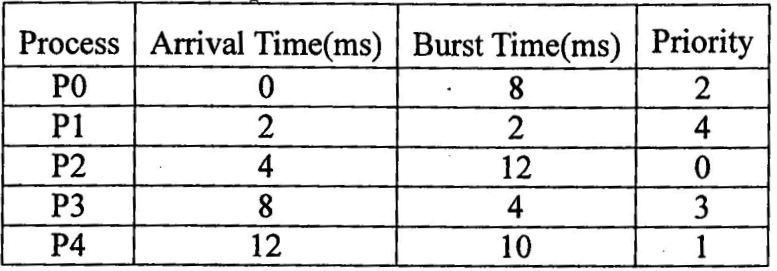
\includegraphics[width=3.5in]{./pics/os_26}
		
			\item Consider the following set of processes, with length of the CPU burst time given in milliseconds. \hfill [8] (\bo{\texttt{81 Bh}, 77 Ch})\\
			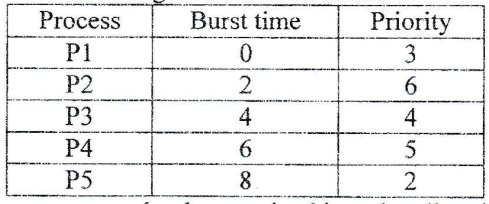
\includegraphics[width=3.5in]{./pics/os_1}\\
			A. All the processes are assumed to have arrived in order all at time 0.
			\begin{enumerate}[noitemsep, topsep = 0pt, label = \alph*.]
				\item Draw Gantt Chart Using FCFS, SJF scheduling algorithm.
				\item Find average turnaround time for each scheduling algorithm.
			\end{enumerate}
			B. Draw Gantt chart illustrating RR (quantum = 2) and highest ratio next (HRN) scheduling. Also find average waiting and average turn around time for each of the algorithm.
			
			\item Schedule the following set of process according to Round-Robin scheduling algorithm with Quantum time = 4ms and calculate the average waiting time and average Turn-around time, throughput and CPV utilization. \hfill [3] (\texttt{81 Ba})\\
			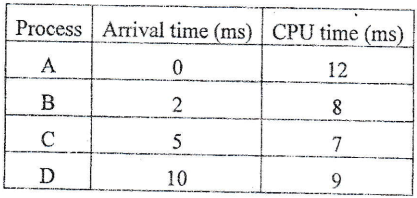
\includegraphics[width=3.5in]{./pics/os_2}
			
			\item Consider the following set of processes, with length of the CPU burst time given in milliseconds. \hspace{12.9cm} [8] (\bo{80 Ch})\\
			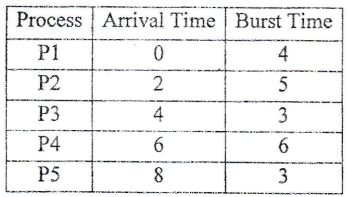
\includegraphics[width=3.5in]{./pics/os_3}\\
			With all the given information, draw the Gantt Chart and calculate the average waiting time (AWT), average turnaround time (ATAT), CPU utilization and throughput for the
			\begin{enumerate}[noitemsep, topsep = 0pt, label = \alph*.]
				\item Round Robin (RR) (Quantum Time = 2)
				\item Highest Response Ratio Next (HRRN)
			\end{enumerate}
			
			\item Make  schedule for the processes mentioned in the table below as per Shortest Remaining Time First (SRTF) algorithm. Also calculate average turnaround time and average waiting time, throughput and CPU utilization. \hfill [6] (\bo{\texttt{80 Bh}})
			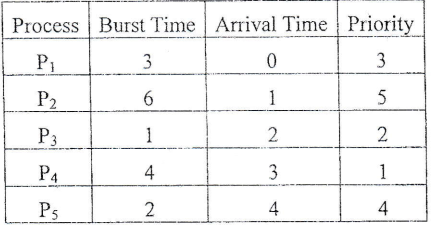
\includegraphics[width=3.5in]{./pics/os_4}
			
			\item Apply MLQ scheduling for following set of processes of two queues Q1 and Q2 where Priority of Q1 is greater than that of Q2 and Q1 uses Round Robin (Time Quantum = 2) and Q2 uses FCFS. Construct Gantt-Chart and computer average TAT for above scenario.
			\enter \hfill [4] (\texttt{80 Ba})\\
			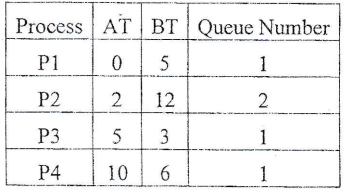
\includegraphics[width=3.5in]{./pics/os_5}
			
			\item Consider following set of process with given arrival and CPU burst time. Calculate the average waiting time for each of process for non-primitive shortest job first (SJF) and Round Robin Scheduling Algorithms with quantum size 4. \hfill [5] (\bo{79 Ch})\\
			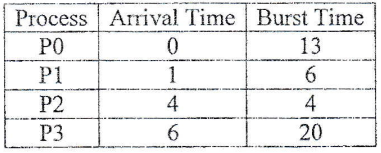
\includegraphics[width=3.5in]{./pics/os_6}
			
			\item Consider the following set of processes, with arrival time and the length of CPU burst time given in millisecond as below: \hfill [6] (76 Ba)\\
			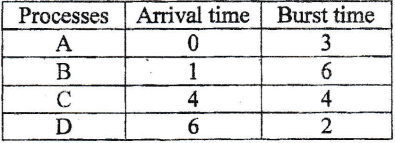
\includegraphics[width=3.5in]{./pics/os_10}\\
			\begin{enumerate}[noitemsep, topsep = 0pt, label = \alph*.]
				\item Draw Gantt chart illustrating the execution of these processes using FCFS, SRTN and RR (Quantum = 2) scheduling.
				\item What is the waiting time and Turnaround time of each process for each of th escheduling algorithm?
			\end{enumerate}
			
			\item Let us consider five process with given arrival time and length of the CPU burst given in milliseconds. Calculate the turnaround time and waiting time for all processes applying First Come First Serve, Shortest Job first and Round Robin (time quantum = 3) algorithms.\\
			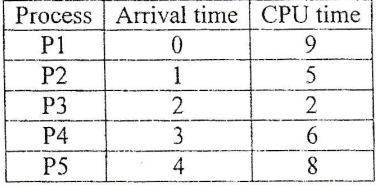
\includegraphics[width=3.5in]{./pics/os_8}
			\hfill [6] (\bo{\texttt{79 Bh}})
			
			\item Assume the process arrived in the order p\sub{1}, p\sub{2}, p\sub{3}, p\sub{4} and p\sub{5} all time 0, priority 1 as highest and 4 as lowest. \hfill [8] (\bo{78 Ch})\\
			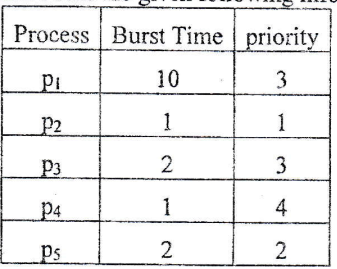
\includegraphics[width=2in]{./pics/os_7}
			\begin{enumerate}[noitemsep, topsep = 0pt, label = \alph*.]
				\item Draw the gantt chart
				\item Calculate average waiting time and average turnaround for the following scheduling algorithm.\\
				i. Round robin (quantum = 1)\\
				ii. priority preemptive\\
				iii. preemptive SJF\\
				iv. FCFS
			\end{enumerate}
			
			\item Consider the following processes, with the length of the CPU burst time in millisecond. The processes are assumed to have arrived in the order P1, P2, P3, P4, P5 all at time 0. [Lowest number being Highest Priority] \hfill [6] (\bo{75 Bh})\\
			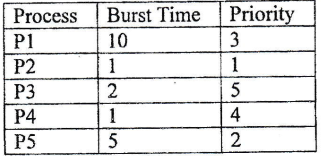
\includegraphics[width=3.5in]{./pics/os_11}\\
			Draw Gantt chart illustrating priority and RR (quantum = 1) scheduling. Also find average waiting time and average turn-around time for each of the algorithms.
			
			\item Consider the following set of processes, with arrival time and the length of CPU burst time given in millisecond as below: \hfill [4+4] (\bo{76 Bh})\\
			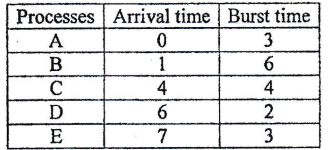
\includegraphics[width=3.5in]{./pics/os_9}
			\begin{enumerate}[noitemsep, topsep = 0pt, label = \alph*.]
				\item Draw Gantt chart illustrating the execution of these processes using FCFS, SRTN and RR (Quantum = 3) scheduling.
				\item What is the waiting time and Turnaround time of each process for each of the scheduling algorithm?
			\end{enumerate}
			
			\item Consider the following set of processes, with the length of the burst time given in milliseconds: (Assume the system has two processors P\sub{1} and P\sub{2}). \hfill [8] (75 Ba)\\
			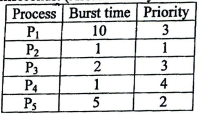
\includegraphics[width=3.5in]{./pics/os_12}\\
			The processes are assumed to have arrived in order p1, p2, p3, p4, p5 all at time 0. Compute the AWT and ATAT for each of the scheduling algorithms. (1) FCFS (2) SJF (3) Pre-emptive priority (4) RR (q=1) scheduling.
			
			\item Suppose 5 processes are submitted at time 0.\\
			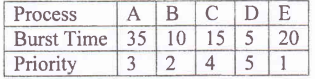
\includegraphics[width=3.5in]{./pics/os_13}\\
			Show the execution timeline of the process using Gantt Chart for FCFS, SJF and Round Robin (q=5). Also calculate mean turnaround time in each case. \hfill [6] (\bo{74 Bh})
			
			\item Make a schedule as per Rate Monotonic (RM) algorithm for the following set of real time tasks:\hfill [5] (73 Ma)\\
			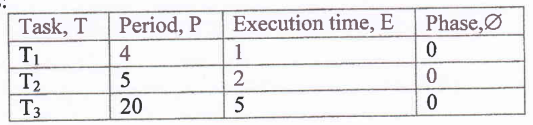
\includegraphics[width=3.5in]{./pics/os_14}
			
			\item Assume the system having two processors of same configuration, schedule the following set of processes according to preemptive priority and round robin algorithm (quantum = 3) and calculate average waiting time and average turnaround time. \hfill [5+5] (\bo{73 Bh})
			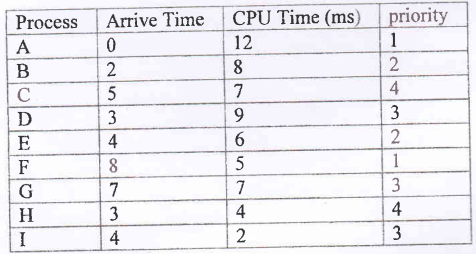
\includegraphics[width=3.5in]{./pics/os_15}
			
			\item Assume you have the following processes to execute with one processor. \hfill [5] (72 Ma)\\
			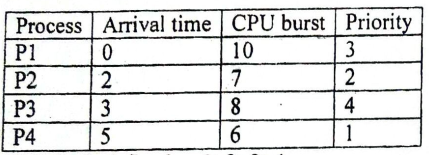
\includegraphics[width=3.5in]{./pics/os_16}\\
			Priority is defined as \( 1 > 2 > 3 > 4 \)\\
			i) Make the GANTT chart of the execution of these using preemptive priority and shortest remaining time first algorithm.\\
			ii) Find out turnaround time, waiting time, and their average time of each process.
			
			\item Schedule the following set of processes according to HRRN and Round Robin algorithm (Time quantum = 4) and calculate average waiting time and average turnaround time. 
			\enter\hfill [5] (\bo{72 Ash})\\
			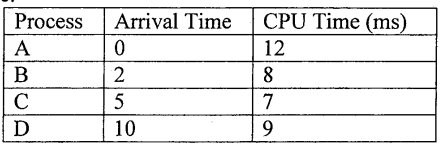
\includegraphics[width=3.5in]{./pics/os_17}
			
			\item From the given following information: \hfill [5] (71 Ma)\\
			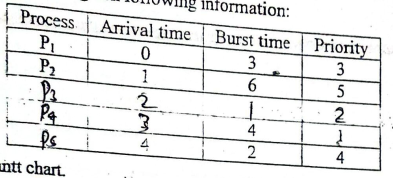
\includegraphics[width=3.5in]{./pics/os_18}\\
			a) Draw the Gantt Chart.\\
			b) Calculate average waiting time and average turn around time for the following scheduling algorithm.\\
			i) Round Robin (q=1) \hspace{1cm} ii) Priority Preemptive \hspace{1cm} iii) Preemptive SJF
			
			\item Schedule the following set of process according to multilevel feedback queue scheduling algorithm and compute AWT and ATAT. \hfill [5] (\bo{71 Bh})\\
			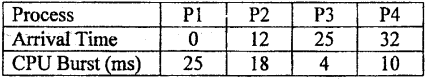
\includegraphics[width=3.5in]{./pics/os_19}\\
			Assume that there are three ready queues Q1, Q2 and Q3. The CPU time slice for Q1 and Q2 is 5 ms and 10 ms respectively and processes are scheduled on FCFS basis in Q3.
			
			\item For the process listed in following table, what is the average turnaround time using: \\
			a) FCFS \hspace{6mm} b) RR (quantum = 4) \hspace{6mm} c) SJF \hspace{6mm} d) SRT \hspace{6mm} e) HRRN \hfill [10] (70 Ma)\\
			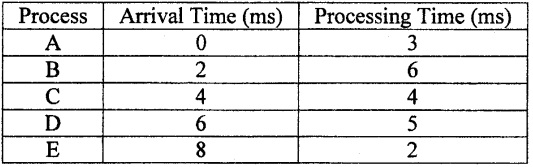
\includegraphics[width=3.5in]{./pics/os_20}
			
			\item Consider the following set of process with the length of the CPU burst time given in millisecond. \hfill [4+4] (\bo{70 Bh})
			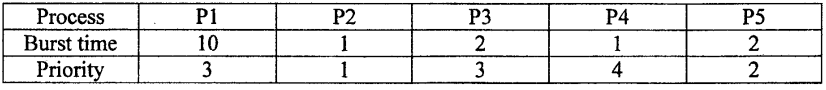
\includegraphics[width=6in]{./pics/os_21}\\
			Assume the processes arrived in the order P1, P2, P3, P4 and P5 all at time 0, priority 1 as highest and 4 as lowest.\\
			a. Draw the Gantt chart for FCFS, SJF, Priority and Round Robin (Quantum = 2)\\
			b. Which algorithm results in the maximum average waiting time?
			
			\item Assume you have the following jobs to execute with one processor. \hfill [6] (68 Ma)\\
			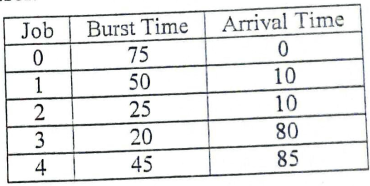
\includegraphics[width=3.5in]{./pics/os_22}\\
			Suppose a system uses round-robin scheduling with quantum of 15 sec.\\
			a. Draw the Gantt chart.\\
			b. Find the average wait and turnaround time.

			\item Schedule the following process applying highest response ratio hext scheduling algorithm. Assume P\sub{1} is the first process. If P\sub{4} need 2 second of service time does the sequence of schedule change? \hfill [7] (\bo{67 Mng})\\
			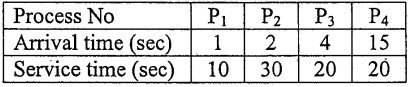
\includegraphics[width=3.5in]{./pics/os_24}
		\end{enumerate}

	\pagebreak
\section{Process Communication and Synchronization}
	\begin{center}(5 Hours/10 Marks)\end{center}
	\subsection{Principles of Concurrency}
		\begin{enumerate}[noitemsep, topsep=0pt]
			\item What is the need process synchronization? \hfill [2] (\bo{\texttt{80 Bh}}, \texttt{80 Ba}, 72 Ma)
		\end{enumerate}
		
	\subsection{Critical Region}
		\begin{enumerate}[noitemsep, topsep=0pt]
			\item Define critical section (\bo{CS}).  \hfill [1] (\bo{65 Ch})
			\lb with respect to multiple-process system. \hfill [1.5] (70 Ma)
			\lb What is CS Problem? \hfill [2] (\bo{80 Ch, 78 Ch, 75 Bh, 73 Bh, 70 Bh}, 76 Ba)

			\item What requirements should be met by solution for . \hfill [2] (76 Ba)
			
			\item Why do we need pipe() function? \hfill [3] (71 Ma)
			
			\item Why is it important for a thread to execute a CS as quickly as possible? \hfill [3] (\bo{73 Bh})
		\end{enumerate}
		
	\subsection{Race Condition}	
		\begin{enumerate}[noitemsep, topsep=0pt]
			\item Define race condition? \hfill [1] (\bo{79 Ch}, 75 Ba) [2] (\bo{79 Bh, 74 Bh, 70 Bh}, 73 Ma)
			\lb with example. \hfill [3] (\bo{71 Bh})

			\item How does a race condition arrive in IPC? \hfill [2] (\bo{77 Ch})
			
			\item What requirements should be met by race condition's solution? \hfill [2] (76 Ba) [3] (75 Ba)
			
			\item Explain disabling interrupts helping to avoid race conditions with drawbacks. \hfill [8] {\small (\bo{66 Ma})}
		\end{enumerate}
		
	\subsection{Mutual Exclusion}
		\begin{enumerate}[noitemsep, topsep=0pt]
			\item What is Mutual Exclusion? \hfill [1] (\bo{79 Ch}, 75 Ba, 65 Ch) [2] (\bo{\texttt{79 Bh}})
			
			\item Define critical section with respect to multiple-process system. \hfill [1.5] (70 Ma)
			
			\item Why must the executing the critical section be mutually exclusive? \hfill [2] (\bo{78 Ch, 75 Bh})
			
			\item What are the requirements of mutual exclusion? \hfill [2] (\bo{\texttt{79 Ch}}, 73 Ma)
			\lb What are conditions to get mutual exclusion? \hfill [2] (\bo{69 Bh})
			
			\item Explain about lock variable for achieving Mutual Exclusion. \hfill [2] (\bo{\texttt{81 Bh}})
			
			\item Explain Peterson's Solution in mutual exclusion.
			\enter\hfill [3] (\texttt{80 Ba}) [4] (76 Ba, 71 Ma) [6] (\bo{\texttt{79 Bh}}) [7] (\bo{71 Bh})
			
			\item Explain how Sleep() and Wakeup() solution is better than busy waiting solution for critical section problem. \hfill [3] (\bo{79 Ch, 74 Bh})
		\end{enumerate}
		
	\subsection{Semaphores and Mutex}
		\begin{enumerate}[topsep=0pt]			
			\item What is is Semaphore? \hfill [1] (\bo{73 Bh, 69 Bh}, \texttt{82 Ba, 80 Ba}, 65 Ka)

			\item Write short notes on Semaphore \hfill [5] (\bo{77 Ch})
			
			\item What is the use of semaphores in IPC. Explain with an example. \hfill [2] (65 Ka)
			\lb How semaphore is used in process synchronization? \hfill [1] (\bo{79 Ch}, \texttt{81 Ba})
			\lb How can semaphore be used to enforce mutual exclusion? Give example. \hfill [5] (75 Ba)
			\lb Describe how semaphore can be used to solve the critical section problem. \hfill [4] (\bo{75 Bh})
			
			\item Explain major operations in semaphore. \hfill [4] (71 Ma)
			\lb including pseudocode. \hfill [5] (\bo{73 Bh})			
			\lb with a simple implementation as a class. \hfill [3] (\bo{74 Bh})
			
			\item Explain the types of semaphore along with major operations of semaphore with a simple pseudocode. \hfill [5] (\bo{\texttt{81 Bh}})
			
			\item Can semaphores be used in distributed system? Explain why or why not? \hfill [3] (71 Ma)
		\end{enumerate}
		
	\subsection{Test and Set Lock, Message Passing \& Monitors}
		\begin{enumerate}[topsep=0pt]
			\item What is TSL (instruction) and why is it used? \hfill [1+1] (\bo{74 Bh}) [2+2] (\bo{72 Ash})
			
			\item Explain TSL approach used in mutual exclusion with busy waiting. \hfill [4] (72 Ma)
			
			\item What makes the message passing IPC as one among the best method of IPC implementation? Explain with pseudo code details. \hfill [10] (70 Ma)
			
			\item What is a monitor? \hfill [2] (\bo{68 Bh})
			
			\item Compare and contrast between monitor and semaphore. \hfill [2.5] (70 Ma) [4] (\bo{76 Bh})
		\end{enumerate}
		
	\subsection{Classical Problems of Synchronization: Readers-Writers Problem, Producer Consumer Problem, Dining Philosopher problem}
		\begin{enumerate}[topsep=0pt]
			\item Explain how semaphore is best solution for producer consumer problem of both producer and consumer process. \hfill [4] (\bo{79 Ch}, \texttt{80 Ba}) [6] (\bo{78 Ch})
			\lb with pseudo-code. \hfill [6] (\bo{80 Ch}) [7] (\texttt{81 Ba})
			
			\item Solve producer and consumer problem using 
			\lb semaphore. \hfill [5] (70 Ma) [6] (\bo{65 Ch}) [7] (\bo{69 Bh}) 
			\lb monitors. \hfill [7] (\bo{72 Ash})
			\lb semaphore and message passing. \hfill [6] (73 Ma)
			
			\item Solve the reader-writer problem with pseduo-codes using semaphore. \hfill [5] (\texttt{82 Ba}) [6] (\bo{\texttt{80 Bh}})
			
			\item Explain dining philosopher problem. \hfill [3] (68 Ma) [3.5] (73 Ma)
			
			\item How can dining philosopher problem be solved? \hfill [5] (68 Ma)
			\lb Explain using any one technique with pseduocode. \hfill [4] (\bo{76 Bh})
			\lb using semaphore. \hfill [5] (\bo{67 Mng}) [6] (\bo{68 Bh})
			
			\item Explain the Sleeping Barber problem and how it occurs. \hfill [1+1] (\bo{77 Ch})
			
			\item Write a solution using any type of your own technique to Sleeping Barber with pseudocode example. \hfill [6] (\bo{77 Ch})
			
			\item Explain all possible approaches to handle the situation ``while one process is busy updating shared memory, no other process will enter its critical section and cause trouble".
			\enter\hfill [8] (\bo{70 Bh})
		\end{enumerate}

	\pagebreak

\section{Memory Management}
	\begin{center}(6 Hours/10 Marks)\end{center}
	\subsection{Managing Free Memory Space}
		\begin{enumerate}[noitemsep, topsep=0pt]
			\item What are the strategies for memory management? \hfill [1] (\bo{79 Ch})
			
			\item Explain free space management techniques for disks.
			\enter\hfill [4] (\bo{71 Bh}) [6] (\bo{72 Ash}, 73 Ma, 70 Ma) [7] (\texttt{80 Ba})
		\end{enumerate}

	\subsection{Resident Monitor, Virtual Memory Management \& Performance}
		\begin{enumerate}[noitemsep, topsep=0pt]
			\item What is resident monitor? \hfill [5] (71 Ma)
			
			\item How is virtual memory management done? \hfill [2] (\bo{\texttt{81 Bh}})

			\item Compare Real Memory and virtual memory. \hfill [2.5] (70 Ma)

			\item What is the impact of size of page in virtual memory management performance? \hfill [2] (75 Ba)
		\end{enumerate}
	
	\subsection{Memory Allocation Techniques}
		\subsubsection{Contiguous: Fixed and Variable}
			\begin{enumerate}[noitemsep, topsep=0pt]
				\item What are the differences of fixed and variable partitioning system of memory for multiprogramming? \hspace{10.6cm} [3] (\bo{75 Bh}, \texttt{81 Ba})

				\item Define internal and external fragmentation. \hfill [2] (75 Ba)

				\item Differentiate between internal and external fragmentation? \hfill [2] (\bo{79 Ch})

				\item Write short ntoes on: Compaction. \hfill [3] (\bo{\texttt{81 Bh}}, \texttt{82 Ba})
				
				\item Write short notes on: Compaction \& Coalescing. \hfill [3] (\bo{80 Ch})
				\lb Differentiate Compaction \& Coalescing. \hfill [2] {\footnotesize (\bo{77 Ch, 73 Bh})} [2.5] {\footnotesize (70 Ma)} [4] {\footnotesize (\bo{\texttt{79 Bh}, 71 Bh})}
				\lb Difference with example. \hfill [4] (75 Ba)
		
				\item Explain first fit, Next fit memory allocation algorithm with an example. \hfill [5] (\texttt{81 Ba})

				\item Explain Best fit and Worst fit memory allocation algorithm with an example. \hfill [5] (\bo{\texttt{80 Bh}})
			\end{enumerate}
			
			\subsubsection{Non-Contiguous: Paging/Segmentation}
				\begin{enumerate}[topsep=0pt]
					\item What is paging? \hfill [1] (70 Ma) [2] (\bo{67 Mng})
					\lb How does paging work? \hfill [2] (70 Ma)
					
					\item What is TLB? \hfill [1] (75 Ba)
					\lb What is the role of TLB? \hfill [2] (\bo{71 Bh})

					\item Prepare a comparative note on: Virtual memory management using Paging versus using Segmentation. \hfill [4] (\bo{76 Bh})
				
					\item Explain how a logical address is mapped to a physical address in paging. \hfill [4] (\bo{\texttt{81 Bh}, 71 Bh})
				\lb with example. \hfill [3] (\bo{73 Bh})

					\item What is segmentation? \hfill [3] (\bo{68 Bh})
				
					\item What is Demand paging? \hfill [1] (\bo{80 Ch, 77 Ch, 72 Ash}) [2] (\bo{78 Ch, 76 Bh})
					
					\item Define page fault. \hfill [2] (\bo{78 Ch, 72 Ash, 79 Bh}, 72 Ma, 70 Ma)
					\lb Under what condition do page fault occur? \hfill [4] (73 Ma)

					\item Why multilevel paging is required? \hfill [2] (\texttt{80 Ba})
					
					\item What is thrashing? \hfill [1] (\bo{77 Ch}, 75 Ba) [2] (\bo{74 Bh, 73 Bh})
					\lb Write short notes on: Thrashing. \hfill [3] (\bo{\texttt{81 Bh, 80 Bh}}) [4] (\bo{75 Bh})
				\end{enumerate}
		
	\subsection{Page Replacement Algorithms}
		\begin{enumerate}[noitemsep, topsep=0pt]
			\item Write short notes on: Belady's anomaly. \hfill [3] (\bo{\texttt{81 Bh}, 80 Ch})
			\lb What is Belady's anomaly in FIFO? \hfill [1] (\bo{\texttt{80 Bh}})
			\lb With example, show that FIFO algorithm suffers from Belady's anomaly. \hfill [3] (\bo{73 Bh})



			\item What is optimal page replacement algorithm? \hfill [2] (68 Ma)

			\item What are the limitation of optimal page replacement. \hfill [4] (\bo{68 Bh})

			\item What is LRU algorithm? \hfill [2] (68 Ma)
		\end{enumerate}
		
	\subsection{Numericals}
		\begin{enumerate}
			\item How many pages fault for the following given reference string for four-page frames 0, 9, 0, 1, 8, 1, 8, 7, 8, 7, 1, 2, 8, 2, 7, 8, 2, 2, 8, 3. \hfill [7] (\bo{\texttt{81 Bh}})\\
			a. LRU\\
			b. FIFO\\
			c. Optimal page
			\lb only Optimal page replacement. \hfill [5] (\bo{75 Bh}, \texttt{81 Ba})

			\item Consider the following page reference Strings; 2, 3, 4, 2, 1, 3, 7, 5, 4, 3, 1, 5. Find how many page faults occur according to optimal, LRU and LFU page replacement algorithm assuming 3-page frames. \hfill [6] (\bo{80 Ch}, \texttt{82 Ba})
			
			\item Consider the following page reference strings: 2, 3, 4, 2, 1, 3, 5, 4, 3, 1, 5, 3, 4, 5, 0, 1, 4, 2. Find how many page fault occur according to Optimal, LRU and LFU page replacement algorithm assuming 3 page frames. \hfill [7] (\bo{\texttt{80 Bh}})

			\item Consider the following page reference string: 5, 0, 2, 1, 0, 3, 2, 4, 3, 0, 3, 2, 1, 3, 0, 1, 5.\\
			Calculate page hit percentage. How many page faults would occur for the FIFO, Optimal, LFU and LRU replacement algorithms having four frames? Remember all frames are initially empty, so your first unique page will cost one fault each. \hfill [8] (\texttt{80 ba})

			\item Consider the following page-reference string 1, 2, 3, 4, 2, 1, 5, 6, 2, 1, 2, 3, 7, 6, 3, 2, 1, 2, 3, 6. How many page faults would occur for LRU and FIFO replacement algorithm assuming 4 frames. \hfill [4] (\bo{79 Ch})
			\lb for 3 frames and LRU, FIFO and Optimal algorithm. \hfill [6] (73 Ma) [8] (72 Ma)
			\lb for 5 frames, for FIFO, Optimal, LFU and LRU replacement. \hfill [8] (70 Ma)

			\item Consider the following page reference strings: 2, 3, 4, 2, 1, 3, 7, 5, 4, 3, 1, 5. Find how many page fault occur according to Optimal, LRU and LFU page replacement algorithm assuming 3 page frames. \hfill [5] (\bo{77 Ch})

			\item Consider the following page-reference storing-\\
			7, 0, 1, 2, 0, 3, 0, 4, 2, 3, 0, 3, 2, 1, 2, 0, 1, 7, 01. How many page faults would occur for the following page replacement algorithms, assuming 3 frames:-\\
			FIFO, Optimal, LRU, LFU. \hfill [8] (\bo{74 Bh})

			\item Calculate Hit and Faults using various page replacement algorithm policies. (FIFO, LRU, Optimal) for the following page sequence of frame size 3: \hfill [2+6] (\bo{70 Bh})\\
			2, 3, 5, 4, 2, 5, 7, 3, 8, 7

			\item How many page faults would occur for the following reference string for page frames using LRU algorithm. \hfill [6] (69 Ma)\\
			1, 2, 3, 4, 5, ,5 3, 4, 1, 6, 7, 8, 7, 8, 9, 5, 4, 5, 4, 2

			\item Consider a swapping system in which memory consists of the following hole sizes in memory order: 10 MB, 4 MB, 20 MB, 18 MB, 7 MB, 9 MB, 12 MB and 15 MB. Which hole is taken for successive segment requests of: \hfill [6] (\bo{\texttt{79 Bh}})\\
			a. 12 MB\\
			b. 10 MB\\
			c. 9 MB\\
			for first fit? Now repeat the question for best fit and worst fit.
			\lb for first, next fit and best fit. \hfill [6] (\bo{67 Mng})

			\item Consider logical address spaces of eight pages of 1024 words, each mapped onto a physical memory of 32 frames then, \hfill [6] (\bo{78 Ch})\\
			a. How many bits are in logical address and physical address?\\
			b. How paging will be done?

			\item Suppose that we have memory of 1000 KB with 5 partitions of size 150 KB, 200 KB, 250 KB, 100 KB and 300KB. Where the processes A and B of size 175 KB and 125 KB will be loaded, if we used Best-Fit and Worst-Fit strategy? \hfill [5] (\bo{79 Ch})

			\item Consider a paged memory system with eight pages of 8KB page size each and 16 page frames in memory. Using the given page table, compute the physical address for the logical address 18325. \hfill [6] (\bo{72 Ash})\\
			\begin{tabular}{|c|c|}
				\hline
				7 & 10 \\ \hline
				6 & 4 \\ \hline
				5 & 0 \\ \hline
				4 & 7 \\ \hline
				3 & 13 \\ \hline
				2 & 11 \\ \hline
				1 & 14 \\ \hline
				0 & 5 \\ \hline
			\end{tabular}

			\item Consider logical address of eight pages of 1024 words, each mapped onto a physical memory of 32 frames. Then, \hfill [5] (71 Ma)\\
			a. How many bits are in logical address?\\
			b. How many bits are in physical address?

			\item Assume that a virtual memory of size 64K is mapped to physical memory of 32K wiht page frame 4K. Initially, pages are mapped as: 0, 1, 2, 3, 4, 5, 9, 11 correspond to 2, 1, 6, 0, 4, 3, 5, 7 respectively. Calculate outgoing physical address for incoming virtual address 20482 with necessary mapping diagram. \hfill [8] (\bo{69 Bh})

			\item Suppose that a total of 64 MB memory is available in a system. This memory space is partitioned into 9 fixed size slots of 8 MB each. Assume 8 processes are currently requesting memory usages with size indicated below. \hfill [6] (68 Ma)\\
			2MB, 4MB, 3MB, 7MB, 9MB, 1MB, 8MB\\
			Calculate the size of memory wasted due to external and internal fragmentation and memory utilization ratio.

			\item Suppose a machine has 48 bit virtual addresses and 32 bit physical address. \hfill [5] (\bo{68 Bh})\\
			a. If pages are 4KB, how many entries in the page table?\\
			b. Suppose the same system has a TLB with 32 entries. Furthermore suppose that a program contains instruction that fit into one page and it sequentially reads long integer elements from an array that spans thousands of pages. How effective will the TLB for this case?
		\end{enumerate}
		
	\subsection{Miscellaneous}
		\begin{enumerate}[topsep=0pt]
			\item (Assumed) What is associative memory\hfill [1] (\bo{77 Ch})
		\end{enumerate}

	\pagebreak

\section{File Systems}
	\begin{center}(6 Hours/10 Marks)\end{center}
	\subsection{File: System, Attribute, Roles, Directory, Path}
		\begin{enumerate}[noitemsep, topsep=0pt]
			\item (Assumed) What are the requirements of long term information storage? \hfill [2] (\bo{67 Mng})

			\item What is file? \hfill [2] (71 Ma)
			
			\item Describe File System for operating system. \hfill [1] (\bo{77 Ch}) [2] (\bo{76 Bh}) [4] (\bo{80 Ch})

			\item What is file attribute? \hfill [1] (\bo{79 Ch}, \texttt{81 Ba}, 75 Ba, 73 Ma, 71 Ma) [2\ (\texttt{82 Ba})
			\lb List out some attributes of file. \hfill [2] (\bo{77 Ch})

			\item What are the major operations required in any file? \hfill [2] (\bo{76 Bh})

			\item What is the role of file system? \hfill [2] (\bo{78 Ch})

			\item What is the role of each layer in file system? \hfill [4] (72 Ma)
			
			\item Define directory. \hfill [1] (76 Ba)
			
			\item What is directory organization in files? Explain its types. \hfill [8] (\bo{\texttt{80 Bh}})

			\item How is file different than Directory? \hfill [2] (\bo{76 Bh})\item Write the difference between Single level directory system and Hierarchial directory system.
				\enter\hfill [3] (73 Ma)
			
			\item Define file path. \hfill [1] (76 Ba)

			\item Differentiate between relative and absolute pathnames. \hfill [3] (\bo{77 Ch})
		\end{enumerate}

	\subsection{File System Implementation}
		\subsubsection{File System Layout}
			\begin{enumerate}[noitemsep, topsep=0pt]
				\item What is file system layout? \hfill [3] (\bo{72 Ash, 68 Bh}) [5] (68 Ma)
				\lb Explain file system layout in detail. \hfill [6] (\bo{70 Bh})

				\item What are the major differences between file system interfaces and file system implementation?
				\enter\hfill [4] (\bo{70 Bh})
			\end{enumerate}

		\subsubsection{Implementing File: Contiguous Allocation, Link List Allocation, Link List Allocation with Table, Inode}
			\begin{enumerate}[noitemsep, topsep=0pt]
				\item Explain various ways of implementing file system. \hfill [6] (\bo{\texttt{79 Bh}}, 75 Ba)

				\item Suggest which implementation of file system is better and why? \hfill [1] (75 Ba)

				\item Explain the file allocation methods. \hfill [2] (70 Ma) [3] (\texttt{80 Ba}) [6] (\bo{71 Bh}) [7] (71 Ma)
				\lb with its adv and disadv. \hfill [5] (\texttt{81 Ba}) [6] (\bo{79 Ch})
				\lb with its adv and disadv and suitable diagram. \hfill [6] (\texttt{82 Ba})
				\lb and access methods with adv and disadv. \hfill [4+6] (\bo{74 Bh})

				\item What is I-node? \hfill [3] (\bo{67 Mng})

				\item Explain I-node approach of file implementation with its adv and disadv.
				\enter\hfill [5] (\bo{\texttt{81 Bh}}) [6] (76 Ba) [8] (75 Bh)

				\item Explain about I-node and file system backup. \hfill [5] (\bo{68 Bh})

				\item Suggest which file organization technique is most appropriate for "tape storage".
				\enter\hfill [1] (\bo{79 Ch})

				\item List any three of them with advantages and disadvantages of each. \hfill [6] (\bo{78 Ch})

				\item Prepare a comparative note on: File implementation using 'Linked list Allocation with Table' versus I-node. \hfill [4] (\bo{76 Bh}) [5] (72 Ma)

				\item How file system is implemented using linked list? \hfill [4] (\bo{69 Bh})

				\item Draw the block diagram of virtual file system? \hfill [3] (\bo{67 Mng})
			\end{enumerate}					
		
		\subsubsection{Impact of Block Size Selection}
			\begin{enumerate}[noitemsep, topsep=0pt]
				\item Explain impact of block size selection on data rate and disk space utilization with necessary diagram and illustration. \hfill [6] (\bo{69 Bh})
			\end{enumerate}
		
	\subsection{File System Performance}
		\begin{enumerate}[noitemsep, topsep=0pt]
			\item List the File System Performance indicator. \hfill [2] (\bo{79 Ch}, \texttt{81 Ba}, 75 Ba)
			\lb with brief explanation. \hfill [4] (\bo{73 Bh})

			\item How do you measure the file system performance? \hfill [2] (\bo{\texttt{79 Bh}})
			
			\item How can file system performance be increased? \hfill [2] (\bo{\texttt{79 Bh}}, \texttt{82 Ba})
		\end{enumerate}
		
	\subsection{Mapping File Blocks on The Disk Platter}
		\begin{enumerate}[noitemsep, topsep=0pt]
			\item (Assumed) Why are output files for the printer normally spooled on disk before being printed?
			\enter\hfill [2] (\bo{80 Ch})

			\item (Assumed) Prepare a comparative note on: Spooling versus Deadline Scheduling.
			\enter\hfill [4] (\bo{76 Bh})
		\end{enumerate}

	\subsection{Example File Systems: CD ROM file system, MS-DOS file system, Unix File system}
		\begin{enumerate}[noitemsep, topsep=0pt]
			\item Write short notes on: UNIX File System. \hfill [3.5] (\bo{73 Bh}) [5] (\bo{77 Ch})

			\item What are the advantages of UNIX? \hfill [2] (68 Ma)

			\item What are the goals of UNIX? \hfill [2] (\bo{68 Bh, 67 Mng})

			\item Draw the structure of UNIX operating system. \hfill [6] (\bo{67 Mng}, 68 Ma)
		\end{enumerate}

	\pagebreak

\section{I/O Management and Disk Scheduling}
	\begin{center}(4 Hours/7 Marks)\end{center}
	\subsection{Principles of I/O Hardware}
		\begin{enumerate}[noitemsep, topsep=0pt]
			\item Write short notes on: USB Storage. \hfill [4] (\bo{76 Bh})
			
			\item Define/Explain DMA? \hfill [2] (\bo{79 Ch, 70 Bh}) [4] (\bo{67 Mng}) [5] (68 Ma)

			\item How DMA increases the system consistency? \hfill [2] (\bo{76 Bh})
		\end{enumerate}

	\subsection{Principles of I/O Software \& I/O Software Layers}
		\begin{enumerate}[noitemsep, topsep=0pt]
			\item What are the principles of I/O software? Explain its types. \hfill [2] (\bo{78 Ch}) [8] (\bo{\texttt{80 Bh}})
			\lb Short notes on principles of I/O software. \hfill [3] (\texttt{82 Ba}) [3.5] (\bo{73 Bh})

			\item Explain about the device independent I/O Software with example. \hfill [6] (\bo{72 Ash})

			\item What are the functions of device independent I/O software?
			\enter\hfill [2] (\bo{67 Mng}, \texttt{80 Ba}) [4] (\bo{70 Bh})

			\item Explain about programmed I/O. \hfill [2] (\bo{80 Ch})

			\item What are the disadv of Programmed I/O? \hfill [2] (\bo{77 Ch, 70 Bh, 67 Mng})
			
			\item Explain the working of DMA Controller with respective figure. \hfill [4] (\texttt{82 Ba})

			\item Explain how I/O takes place through DMA? \hfill [2] (\bo{79 Ch})

			\item Briefly mention the structured I/O software with suitable diagram. \hfill [3] (\bo{73 Bh})

			\item Explain about device driver structure. \hfill [5] (\bo{67 Mng})

			\item Explain the working of device driver. \hfill [4] (\bo{69 Ch})
		\end{enumerate}
		
	\subsection{Disk}
		\subsubsection{Hardware}
			\begin{enumerate}[noitemsep, topsep=0pt]
				\item What do you mean by RAID? \hfill [2] (\bo{\texttt{79 Bh}})
				
				\item Why do we organize disk as RAID? \hfill [2] (\texttt{81 Ba})

				\item Explain how RAID level 1 differs from RAID level 0? \hfill [2] (\bo{80 Ch})
			\end{enumerate}
		\subsubsection{Formatting}
		\subsubsection{Arm scheduling}
			\begin{enumerate}[noitemsep, topsep=0pt]
				\item Compare the the throughput (overall performance) of SCAN with SSTF. \hfill [3] (\bo{73 Bh})

				\item Write short notes on SSTF algorithm with example. \hfill [4] (72 Ma)

				\item What is disk scheduling? \hfill [3] (\bo{72 Ash})
			\end{enumerate}

		\subsubsection{Error handling}
		\subsubsection{Stable Storage}
	\subsection{Numericals}
		\begin{enumerate}
			\item A disk drive has 50 cylinders, numbered 0 to 49. The drive is currently serving a request at cylinder 15, and the queue of pending requests, in FIFO order is 4, 40, 11, 35, 7, 14. What is the total distance that the disk moves for the following algorithms: \hfill [10] (\bo{74 Bh})\\
			FCFS, SSTF, SCAN, LOOK, C-SCAN.
			
			\item Consider a disk drive having 100 cylinders. The head is currently serving request at cylinder 43 and the previous request was at 56. The queue of pending request is 86, 70, 13, 74, 48, 9, 22, 50, 30. Starting from current head position, what is total head movement (in cylinders) to service the pending requests of each of following disk arm scheduling algorithms.\\
			a. FCFS\\
			b. SSTF\\
			c. SCAN\\
			d. LOOK \hfill [6] (\bo{\texttt{81 Bh}})
			\lb Only FCFS and C-SCAN. \hfill [6] (\bo{\texttt{80 Bh}})
			\lb FCFS, C-SCAN, and SSTF \hfill [6] (\bo{78 Ch})
			\lb FCFS, SSTF, LOOK, C-SCAN, SCAN. \hfill [10] (70 Ma)

			\item Consider a disk drive with 150 cylinders numbered from 0-149. The drive is currently serving a request at 35 and the previous request is at disk 55. The queue of pending request is 98, 103, 38, 122, 10, 128, 65, 75. Starting from the current head position. Calculate the total head moment (in cylinder) that the disk arm moves to satisfy all the pending request for SSF, SCAN and LOOK Disk Arm Scheduling Algorithm. \hfill [6] (\bo{76 Bh}, \texttt{81 Ba})
			\lb for SSTF, SCAN, C-SCAN, LOOK and FCFS. \hfill [10] (75 Ba)
			
			\item Consider a disk queue with requests for IO to blocks on cylinder 175, 155, 188, 23, 169, 15, 130 for cylinders from 0-199 (200 cylinders). The current head is at 100 which had just finished the request at cylinder 109. Starting from the current head position, find total head movement for FCFS, SSTF and SCAN disk arm scheduling algorithm. \hfill [6] (\texttt{72 Ba})
 
			\item Consider a disk queue having 200 cylinders from 0 to 199 with requests for IO to blocks on cylinders are 23, 89, 132, 42 and 187. Assume disk head initially at 100 and a seek takes 6ms/cylinder. How much seek is needed for FCFS, SSTF, SCAN and LOOK disk arm scheduling algorithms? \hfill [8] (\bo{80 Ch})
			\lb for FCFS, SSF and SCAN disk algorithms. \hfill [8] (\bo{{75 Bh}})

			\item Suppose the head of a moving head disk with 200 traks, 0 to 199, is currently serving a request at track 143 and has finished a request at track 125. The queue it requests is kept in FIFO order: 25, 17, 119, 197, 194, 15, 182, 115, 183. What is the total movement needed to satisfy these requestsfor the following disk-scheduling algorithms? \hfill [6] (\bo{79 Ch})\\
			(\textit{no algorithm is listed})

			\item Suppose a disk with 200 cylinders numbered from 0-199. The drive is currently serving a request was at 125. The queue of pending request is 105, 178, 23, 67, 43, 78, 167, 56 and 98. Starting from current head position, calculate the total head movement (in cylinder) that the disk arm moves to satisfy all pending request for SSTF, SCAN, LOOK and C-SCAN disk scheduling algorithm. \hfill [8] (\bo{\texttt{79 Bh}})

			\item Suppose that a disk has 200 tracks, numbered from 0 to 199. The read/write head of drive is currently serving a request at track 143, and has just finished the request at track 125. The queue of pending request in FIFO order is:\\
			86, 147, 91, 177, 94, 160, 102, 175, 130\\
			Suppose seek takes 10ms per cylinder moved. Starting from the current head position, what is the total distance that the disk arm moves to satisfy all the pending request, for FCFS, SSTF, C-SCAN and C-LOOK algorithm? Also calculate seek time needed to serve these request for each algorithm. \hfill [8] (\bo{77 Ch})

			\item Suppose a disk drive with 200 cylinders numbered from 0 to 199. The drive is currently at 53. The queue of pending request is 98, 183, 37, 122, 14, 124, 65, 67. Starting from the current head position, calculate total head movement that the disk arm moves to satisfy all the pending request for FCFS, SSTF and SCAN disk scheduling algorithm.
			\enter\hfill [6] (\bo{69 Bh}, 73 Ma)
			\lb for FCFS, SSTF, SCAN, LOOK, C-SCAN. \hfill [11] (71 Ma)

			\item A disk with 1000 cylinders, numbered 0 to 999, compute the number of tracks the disk arm must move to satisfy all the requests in the disk queue. Assume the last request serviced was at track 345 and the head is moving towards track 0. The queue in FIFO order contains request for the following tracks: \hfill [10] (\bo{71 Bh})\\
			123, 874, 693, 475, 105, 376.\\
			Perform the computation for the following scheduling algorithms:\\
			FIFO, SSTF, SCAN

			\item Suppose that a disk has 5000 cylinders, numbered from from 0 to 4999. The drive is currently serving a request at cylinder 143, and the previous request was at cylinder 125. The queue of pending requests in FIFO order is: \hfill [8] (\texttt{80 Ba})\\
			86, 1470, 913, 1774, 948, 1509, 1022, 1750, 130\\
			Starting from the current head position, what is the total distance (in cylinders) that the disk arm moves to satisfy all the pending requests, for FCFS, SSTF, C-SCAN and C-LOOK Algorithm?
			\lb Queue's head is 56, algorithms: FCFS, SCAN, LOOK, CSCAN, SSTF. \hfill [10] (72 Ma)

			\item Consider a Winchester-style hard disc with 100 cylinders, four double-sided platters and 25 sectors per track. The following is time ordered sequence of requests for disc sectors: {3518, 1846, 8924, 6672, 1590, 4126, 107, 9750, 158, 6621, 446, 11}. The disc arm is currently at cylinder 10, moving to 100. FOr each of SSTF, SCAN, and C-SCAN, give the order in which the above requests would be served? \hfill [6] (\bo{68 Bh})
		\end{enumerate}
		
	\subsection{Miscellaneous}
		\begin{enumerate}[noitemsep, topsep=0pt]
			\item (Assumed) State the advantages and disadvantages of placing the functionality in a device controller than in kernel. \hfill [3] (68 Ma)

			\item (Assumed) What is interleaving? \hfill [2] (\bo{68 Bh})
		\end{enumerate}

\pagebreak
\section{Deadlock}
	\begin{center}(5 Hours/10 Marks)\end{center}
	\subsection{Principles of deadlock \& Other Issues}
		\begin{enumerate}[noitemsep, topsep=0pt]
			\item Define deadlock. \hfill [1] (\bo{74 Bh}, 76 Ba) [2] (\bo{72 Ash, 70 Bh}, 70 Ma)
			
			\item Explain the resource allocation graph with an example. \hfill [2] (\bo{\texttt{81 Bh}, 78 Ch})

			\item Explain necessary conditions for deadlock.
			\enter\hfill [2] {\footnotesize (\bo{80 Ch}, \texttt{81 Ba}, 75 Ba)} [3] {\footnotesize (\bo{74 Bh})} [4] {\footnotesize (\bo{72 Ash, 69 Bh}, \texttt{82 Ba}, 71 Ma)}
			\lb Explain Coffman conditions for deadlock. \hfill [3] (\texttt{80 Ba})
			\lb What are the conditions for resource deadlock? \hfill [2] (76 Ba)
			\lb Explain each condition of deadlock. \hfill [4] (73 Ma)

			\item State the conditions for deadlock to occur and why all conditions are necessary. \hfill [8] (\bo{70 Bh})

			\item How does deadlock occur? \hfill [2] (70 Ma)

			\item How unsafe state differs from deadlock state? \hfill [1] (\bo{79 Ch})

			\item What is indefinite postponement? \hfill [1] (\bo{76 Bh, 74 Bh})
			
			\item Is indefinite postponement different than deadlock? \hfill [3] (\bo{76 Bh, 73 Bh})
		\end{enumerate}

	\subsection{Deadlock Ignorance, Detection \& Recovery}
		\begin{enumerate}[noitemsep, topsep=0pt]
			\item Write short notes on: Ostritch algorithm. \hfill [3] (\texttt{81 Ba})
			
			\item Explain in deatil how can detect deadlock in operating system. \hfill [3] (\bo{79 Ch})

			\item What is deadlock detection? \hfill [1] (72 Ma)

			\item How do you detect deadlock? Explain with example. \hfill [4] (\bo{72 Ash})
			\lb How can a system detect deadlock and what does it do after detection? \hfill [6] (71 Ma)

			\item Explain the algorithm for detecting deadlock for one resource of each type. \hfill [4] (\bo{67 Mng})
			
			\item Explain some methods for recovering from deadlocks? \hfill [5] (76 Ba)

			\item How deadlock is recovered? \hfill [3] (\texttt{82 Ba}, 73 Ma)
		\end{enumerate}

	\subsection{Deadlock Avoidance}
		\begin{enumerate}[noitemsep, topsep=0pt]

			\item Explain various deadlock avoidance methods with examples. \hfill [6] (70 Ma)

			\item What is deadlock avoidance? \hfill [1] (72 Ma)
		\end{enumerate}

	\subsection{Deadlock Prevention}
		\begin{enumerate}[noitemsep, topsep=0pt]
			\item What is deadlock prevention? Explain deadlock prevention techniques? \hfill [5] (\bo{79 Ch})
			\lb Explain all possible deadlock prevention techniques. \hfill [6] (72 Ma)

			\item Explain how deadlock can be prevented? \hfill [3] (\bo{74 Bh})

			\item Explain how you can detect deadlock in operating system. \hfill [3] (\bo{77 Ch})

			\item  What would be necessary to prevent deadlock? \hfill [3] (73 Ma) 
		\end{enumerate}

	\subsection{Numericals}
		\begin{enumerate}
			\item A system has 2 process and 3 resources. Each process needs maximum of two resources, is deadlock possible? Explain. \hfill [2] (\bo{74 Bh}) [3] (\texttt{82 Ba})

			\item Consider the system consists of m resources of same type being shared by n process of which need at most two resource. Explain whether the system is deadlock free or not?
			\enter\hfill [4] (\bo{67 Mng})

			\item Consider the following initial state and identify whether requested resource is granted or denied for given cases. \hfill [4] (\bo{79 Ch})\\
			\begin{tabular}{|c|c|c|}
				\hline
				Process & Has & Max \\ \hline
				A & 2 & 6 \\ \hline
				B & 1 & 5 \\ \hline
				C & 2 & 3 \\ \hline
				D & 3 & 8 \\ \hline
			\end{tabular}\\
			Free Resource = 2\\
			a. What will happen if process A request 1 Resource?
			b. What will happen if process D request 1 Resource

			\item Consider a system with 4 concurrent process (P1, P2, P3, P4) and three source types A, B and C with total instances 7, 10 and 10 respectively. The allocation and maximum claim at state t\sub{0} is: \hfill [8] (\bo{\texttt{81 Bh}})\\
			\begin{tabular}{|p{17mm}|p{7mm}|p{7mm}|p{7mm}|p{7mm}|p{7mm}|p{7mm}|}
				\hline
				\multirow{2}{*}{Processes} & \multicolumn{3}{|c|}{Allocation} & \multicolumn{3}{|c|}{Maximum Claim} \\ \cline{2-7}
				& A & B & C & A & B & C \\ \hline
				P1 & 1 & 2 & 0 & 3 & 5 & 9 \\ \hline
				P2 & 3 & 0 & 2 & 5 & 0 & 5 \\ \hline
				P3 & 1 & 2 & 2 & 2 & 2 & 5 \\ \hline
				P4 & 0 & 4 & 0 & 0 & 10 & 2 \\ \hline
			\end{tabular}\\
			a. What is the total number of available resources?
			b. What will be the need matrix?
			c. Is the system safe? If so, show the sequence.

			\item Consider a system with five processes p0 through p4 and three resource types A, B and C. Resource A has 5 instances, B has 5 instances and C has 4 instances. Suppose at time t = 0, following snapshot has been taken.\\
			\begin{tabular}{|p{17mm}|p{7mm}|p{7mm}|p{7mm}|p{7mm}|p{7mm}|p{7mm}|}
				\hline
				\multirow{2}{*}{Processes} & \multicolumn{3}{|c|}{Allocation} & \multicolumn{3}{|c|}{Maximum Claim} \\ \cline{2-7}
				& A & B & C & A & B & C \\ \hline
				P0 & 0 & 3 & 1 & 3 & 3 & 1 \\ \hline
				P1 & 3 & 2 & 1 & 4 & 2 & 1 \\ \hline
				P2 & 1 & 0 & 1 & 1 & 1 & 1 \\ \hline
				P3 & 0 & 0 & 0 & 2 & 2 & 0 \\ \hline
				P4 & 0 & 0 & 0 & 1 & 0 & 0 \\ \hline
			\end{tabular}\\
			Let the available number of resources be given by available vectors as (1, 0, 1). Is the system in safe state? If yes, then write safe sequence. \hfill [8] (\bo{80 Ch})

			\item Consider the folllowing snapshot: \hfill [7] (\texttt{80 Ba})\\
			\begin{tabular}{|p{17mm}|p{7mm}|p{7mm}|p{7mm}|p{7mm}|p{7mm}|p{7mm}|}
				\hline
				\multirow{2}{*}{Processes} & \multicolumn{3}{|c|}{Allocation} & \multicolumn{3}{|c|}{Maximum Claim} \\ \cline{2-7}
				& A & B & C & A & B & C \\ \hline
				P0 & 0 & 1 & 0 & 7 & 5 & 3 \\ \hline
				P1 & 2 & 0 & 0 & 3 & 2 & 2 \\ \hline
				P2 & 3 & 0 & 2 & 9 & 0 & 2 \\ \hline
				P3 & 2 & 1 & 1 & 2 & 2 & 2 \\ \hline
				P4 & 0 & 0 & 2 & 4 & 3 & 3 \\ \hline
			\end{tabular}\\
			The available resources are A: 3, B: 2, and C: 2. Is the state safe? If so, show the safe execution of processes. \hfill [6] (\bo{78 Ch}) [7] (\texttt{80 Ba}) [8] (75 Ba)

			\item Consider a system with 5 processes P0 through P4 and three resources type A, B and C. Resources A has 7 instances, B has 2 and C has 6 instances. Suppose at time t0 we have following state. \hfill [7] (\bo{77 Ch})\\
			\begin{tabular}{|p{17mm}|p{7mm}|p{7mm}|p{7mm}|p{7mm}|p{7mm}|p{7mm}|}
				\hline
				\multirow{2}{*}{Processes} & \multicolumn{3}{|c|}{Allocation} & \multicolumn{3}{|c|}{Request} \\ \cline{2-7}
				& A & B & C & A & B & C \\ \hline
				P0 & 0 & 1 & 0 & 0 & 0 & 0 \\ \hline
				P1 & 2 & 0 & 0 & 2 & 0 & 0 \\ \hline
				P2 & 3 & 0 & 3 & 0 & 0 & 0 \\ \hline
				P3 & 2 & 1 & 1 & 1 & 0 & 0 \\ \hline
				P4 & 0 & 0 & 2 & 0 & 0 & 2 \\ \hline
			\end{tabular}\\
			a. Is the state safe? If so, show the safe execution of the process.\\
			b. Suppose P2 makes additional request of (1, 0, 1, 0), what will be the effect of this request to the system?

			\item Consider a system with 5 processes and three resources. Resources A has 7, B has 2 and C has 6 instances. Suppose at t0 time we have following state with 0 available A, B and C left:\\
			\begin{tabular}{|p{17mm}|p{7mm}|p{7mm}|p{7mm}|p{7mm}|p{7mm}|p{7mm}|}
				\hline
				\multirow{2}{*}{Processes} & \multicolumn{3}{|c|}{Allocation} & \multicolumn{3}{|c|}{Request} \\ \cline{2-7}
				& A & B & C & A & B & C \\ \hline
				P0 & 0 & 1 & 0 & 0 & 0 & 0 \\ \hline
				P1 & 2 & 0 & 0 & 2 & 0 & 2 \\ \hline
				P2 & 3 & 0 & 3 & 0 & 0 & 0 \\ \hline
				P3 & 2 & 1 & 1 & 1 & 0 & 0 \\ \hline
				P4 & 0 & 0 & 2 & 0 & 0 & 2 \\ \hline
			\end{tabular} \hfill [10] (\bo{71 Bh})\\
			a. Is the given system in deadlock state?\\\
			b. Suppose P2 makes an additional request (0, 0, 1) what will be the effect of this request to this system?

			\item A system has four processes and three resources with existing resource E = (15 9 5). After following allocation, resource available becomes A = (3 2 0). Use Banker's Algorithm to test whether the given state is safe or not. If it is safe state, show the sequence of execution of processes. \hfill [8] (\bo{69 Ch})\\
			\begin{tabular}{|p{17mm}|p{7mm}|p{7mm}|p{7mm}|p{7mm}|p{7mm}|p{7mm}|p{7mm}|p{7mm}|p{7mm}|}
				\hline
				\multirow{2}{*}{Processes} & \multicolumn{3}{|c|}{Allocation} & \multicolumn{3}{|c|}{Maximum} & \multicolumn{3}{|c|}{Need} \\ \cline{2-10}
				& R1 & R2 & R3 & R1 & R2 & R3 & R1 & R2 & R3 \\ \hline
				P1 & 3 & 0 & 1 & 3 & 2 & 2 & 0 & 2 & 1 \\ \hline
				P2 & 5 & 4 & 1 & 6 & 8 & 2 & 1 & 4 & 1 \\ \hline
				P3 & 2 & 2 & 0 & 3 & 2 & 4 & 1 & 0 & 4 \\ \hline
				P4 & 2 & 1 & 3 & 4 & 2 & 3 & 2 & 1 & 0 \\ \hline
			\end{tabular}

			\item Consider a system with 5 concurrent processes (P0, P1, P2, P3, P4) and 4 resource types (R0, R1, R2, R3). The number of instances of each resource type in the system are 6, 4, 4, 2 respectively. Allocation table and maximum claim table are as follows: \\
			\begin{tabular}{|p{17mm}|p{7mm}|p{7mm}|p{7mm}|p{7mm}||p{7mm}|p{7mm}|p{7mm}|p{7mm}|}
				\hline
				\multirow{2}{*}{Processes} & \multicolumn{4}{|c||}{Allocation} & \multicolumn{4}{|c|}{Maximum Claim} \\ \cline{2-9}
				& R0 & R1 & R2 & R3 & R0 & R1 & R2 & R3 \\ \hline
				P0 & 2 & 0 & 1 & 1 & 3 & 2 & 1 & 1 \\ \hline
				P1 & 1 & 1 & 0 & 0 & 1 & 2 & 0 & 2 \\ \hline
				P2 & 1 & 1 & 0 & 0 & 1 & 1 & 2 & 0 \\ \hline
				P3 & 1 & 0 & 1 & 0 & 3 & 2 & 1 & 0 \\ \hline
				P4 & 0 & 1 & 0 & 1 & 2 & 1 & 0 & 1 \\ \hline
			\end{tabular} \\
			a. Calculate Need matrix as per Banker's Algorithm. \hfill [7] (\bo{73 Bh}) [8] (\bo{\texttt{80 Bh}, 76 Bh})\\
			b. Is the state safe? If so, show the safe execution of the processes.
			\lb For P3's R3 Allocation, its 1, rest is same question. \hfill [8] (\bo{76 Bh})

			\item Consider the following snapshot of a system. By using Bankers algorithm, calculate the need matrix. is the system safe? If safe find safe order of process. \hfill [6] (\texttt{80 Ba})\\
			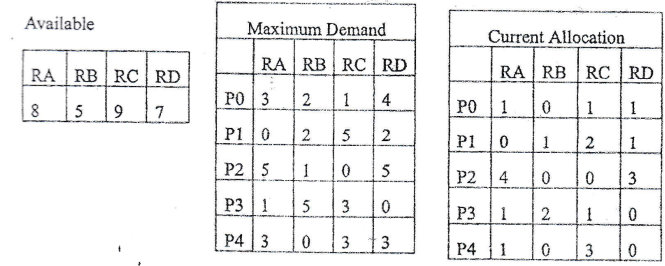
\includegraphics[width=4in]{./pics/os_25}

			\item Consider the following system with resources A, B, C, D and process P0 to P4. Is the state safe? If so, show the safe execution of process. \hfill [7] (\bo{79 Ch})\\
			\begin{tabular}{|p{17mm}|p{7mm}|p{7mm}|p{7mm}|p{7mm}||p{7mm}|p{7mm}|p{7mm}|p{7mm}|}
				\hline
				\multirow{2}{*}{Processes} & \multicolumn{4}{|c||}{Max} & \multicolumn{4}{|c|}{Allocation} \\ \cline{2-9}
				& A & B & C & D & A & B & C & D \\ \hline
				P0 & 6 & 0 & 1 & 2 & 4 & 0 & 0 & 1 \\ \hline
				P1 & 1 & 7 & 5 & 0 & 1 & 1 & 0 & 0 \\ \hline
				P2 & 2 & 3 & 5 & 6 & 1 & 2 & 5 & 4 \\ \hline
				P3 & 1 & 6 & 5 & 3 & 0 & 6 & 3 & 3 \\ \hline
				P4 & 1 & 6 & 5 & 6 & 0 & 2 & 1 & 2 \\ \hline
			\end{tabular}\\
			Available resources are A: 3, B: 2, C: 1, D:1.

			\item A system that uses Banker's Algorithm deadlock avoidance has five processes (1, 2, 3, 4, 5) and four types of resources (A, B, C, D). There are multiple resources of each type. Is the following state safe or not? If it is, show how the processes can complete. If not, show how they can deadlock? \hfill [8] (\bo{68 Bh})
			\begin{tabular}{|p{17mm}|p{7mm}|p{7mm}|p{7mm}|p{7mm}||p{7mm}|p{7mm}|p{7mm}|p{7mm}||p{7mm}|p{7mm}|p{7mm}|p{7mm}|}
				\hline
				\multirow{2}{*}{Processes} & \multicolumn{4}{|c||}{Current Loan} & \multicolumn{4}{|c||}{Max Need} &  \multicolumn{4}{|c|}{Current Claim} \\ \cline{2-13}
				& A & B & C & D & A & B & C & D & A & B & C & D \\ \hline
				1 & 1 & 0 & 2 & 0 & 3 & 2 & 4 & 2 & 2 & 2 & 2 & 2\\ \hline
				2 & 0 & 3 & 1 & 2 & 3 & 5 & 1 & 2 & 3 & 2 & 0 & 0\\ \hline
				3 & 2 & 4 & 5 & 1 & 2 & 7 & 7 & 5 & 0 & 3 & 2 & 4\\ \hline
				4 & 3 & 0 & 0 & 6 & 5 & 5 & 0 & 8 & 2 & 5 & 0 & 2\\ \hline
				5 & 4 & 2 & 1 & 3 & 6 & 2 & 1 & 4 & 2 & 0 & 0 & 1\\ \hline
			\end{tabular}\\
			Available resources are A: 3, B: 4, C: 0, D:1\\
			Total Resources are: A: 13, B: 13, C: 9, D: 13			
		\end{enumerate}

	\pagebreak

\section{Security}
	\begin{center}(4 Hours/7 Marks)\end{center}
	\subsection{Security breaches}
		\begin{enumerate}[noitemsep, topsep=0pt]
			\item Write the type of security breach in following attack case? Also suggest a solution in each to prevent the attack. \hfill [2+2+2] (\texttt{81 Ba})\\
			``Ramesh found that Nirma's facebook was login in Computer Lab. He then changed the personal information and login credentials of Nirmal's account."

			\item What are the security issues associated with OS? Discuss them. \hfill [2] (76 Ba) [4] (\bo{76 Bh})

			\item The use of internet is possible cause of a security breach. Describe the major threats by which a system connected to the internet is always prone to attack. Explain. \hfill [6] (72 Ma)
		\end{enumerate}

	\subsection{Types of Attacks}
		\begin{enumerate}[noitemsep, topsep=0pt]
			\item What are the types of Network Attacks? \hfill [2] (\bo{\texttt{80 Bh}, 79 Ch, 77 Ch})
			\lb Write short notes on: Types of network security attack. \hfill [5] (\bo{71 Bh})

			\item Write short notes on: Types of Security Attack. \hfill [3.5] (\bo{73 Bh})

			\item Write short notes on: Security attack. \hfill [4] (70 Ma)

			\item Explain the types of attacks. \hfill [3] (\bo{72 Ash})

			\item What are the attacks from inside? \hfill [4] (68 Ma)

			\item Explain about Malware and Spyware. \hfill [4] (68 Ma)
		\end{enumerate}

	\subsection{Security Policy and Access Control}
		\begin{enumerate}[noitemsep, topsep=0pt]
			\item Write Short notes on: Security Policy. \hfill [3] (71 Ma)

			\item (Assumed) What is trap door? \hfill [2] (\bo{68 Bh})
		\end{enumerate}

	\subsection{Basics of Cryptography}
		\begin{enumerate}[noitemsep, topsep=0pt]
			\item How does Caesar Cipher convert plain text to ciphertext? \hfill [4] (\bo{\texttt{81 Bh}})

			\item Write short notes on Caesar Cipher. \hfill [3] (\bo{\texttt{79 Bh}, 74 Bh}, \texttt{82 Ba})

			\item Write short notes on: Cryptography. \hfill [2.5] (\texttt{80 Ba}) [3] (71 Ma) [3.5] (73 Ma)

			\item Write short notes on: Public Key Cryptography \hfill [3] (75 Ba) [4] (\bo{78 Ch})

			\item Explain private and public key used in asymmetric cryptography. \hfill [5] (\bo{75 Bh})
		\end{enumerate}

	\subsection{Protection Mechanisms}
		\begin{enumerate}[noitemsep, topsep=0pt]
			\item (Assumed) Write short notes: Protection Domain \hfill [3] (\bo{80 Ch}, 75 Ba) [3.5] (73 Ma)
			\lb Explain protection domain. \hfill [2] (\texttt{82 Ba}) [2.5] (\bo{69 Ch})
			\lb (Assumed) Explain domain-object. \hfill [2] (\bo{70 Bh})

			\item (Assumed) how is domain-object implemented for security? \hfill [2] (\bo{70 Bh})

			\item Write short notes on: Protection matrix. \hfill [2] (\bo{76 Bh})

			\item (Assumed) Why 'HASH' function is called Message Digestor?
			\enter\hfill [1] (\bo{79 Ch}) [2] (\bo{\texttt{80 Bh}, 77 Ch}, \texttt{82 Ba})

			\item (Assumed) What are the roles of system administrator for change management?
			\enter\hfill [4] (\bo{78 Ch})

			\item Explain how you can implement security and protection on all components of a system.
			\enter\hfill [6] (\bo{72 Ash})

			\item (Assumed) Write short notes on: Information security model. \hfill [4] (70 Ma)

			\item (Assumed) Explain about firewalls. \hfill [3] (\bo{68 Bh, 67 Mng})

			\item (assumed) Explain about NFS protocol and draw the structure of NFS. \hfill [6] (\bo{68 Bh})
		\end{enumerate}

	\subsection{Authentication}
		\begin{enumerate}[noitemsep, topsep=0pt]
			\item How authentication is an essential mechanism for maintaining security? Explain.
			\enter\hfill [4] (\bo{74 Bh})
		\end{enumerate}

	\subsection{OS Design Considerations For Security}
	\subsection{Access Control Lists And OS Support}
		\begin{enumerate}[noitemsep, topsep=0pt]
			\item What is ACL?
			\enter\hfill [2] (\bo{\texttt{81 Bh, 80 Bh}, 79 Ch, 77 Ch, 70 Bh}, \texttt{82 Ba, 81 Ba}) [2.5] (\bo{69 Ch}, \texttt{80 Ba}) [3] (\bo{68 Bh})

			\item Write short notes on: Access Control Lists. \hfill [3] (\bo{\texttt{79 Bh}})

			\item Explain ACL with its use in security. \hfill [6] (76 Ba)
			\lb What is the use of ACL? \hfill [3] (\bo{75 Bh})

			\item How is ACL different from the capabilities list? \hfill [2] (\bo{\texttt{81 Bh}})

			\item Describe how Access Control List is used. \hfill [2] (\bo{72 Ch}) [3] (\bo{80 Ch}) [4] (\bo{78 Ch})
		\end{enumerate}

	\pagebreak

\section{System administration}
	\begin{center}(4 Hours/6 Marks)\end{center}
	
	\begin{enumerate}[noitemsep, topsep=0pt]
		\item Write short ntoes on: System administration. \hfill [3.5] (73 Ma)

		\item What is system administration? \hfill [2] (\bo{72 Ash})
		\lb define system adminstrator. \hfill [1] (\texttt{82 Ba})
		
		\item What are the different technical and soft skills that one should pursue as a system adminstrator? \hfill [6] (\texttt{82 Ba})
	\end{enumerate}

	\subsection{Administration Tasks}
		\begin{enumerate}[noitemsep, topsep=0pt]
			\item Write short notes on: Administration tasks. \hfill [3] (\bo{74 Bh})

			\item What are the roles of a system administrator?
			\enter\hfill [2.5] \begin{tiny} (\texttt{81 Ba}) \end{tiny} [3.5] \begin{tiny} (\bo{73 Bh}) \end{tiny} [4] \begin{tiny} (\bo{\texttt{81 Bh}, 76 Bh, 70 Bh}, 75 Ba, 72 Ma, 70 Ma) \end{tiny} [5] \begin{tiny} (\bo{80 Ch, 71 Bh}) \end{tiny} [6] \begin{tiny} (\bo{\texttt{80 Bh}}) \end{tiny}
			\lb Describe the role and responsibilities of a system adminstrator to keep the system updated and efficient. Explain with examples. \hfill [6] (\texttt{81 Ba}, 76 Ba)
			
			\item What is the significance of system administration? Describe the roles and responsibilities of system administrator of Insurance Company. \hfill  [4] (\bo{\texttt{79 Bh}})
			\lb ... adminstrator to keep system updated and efficient. Explain with example.
			\enter\hfill [3+5] (\bo{75 Bh})

			\item How can you increase operating system performance if you are selected as a system adminstrator? \hspace{12.6cm} [4] (70 Ma)

			\item List out some system administration tasks in OS. \hfill [2] (76 Ash)

			\item Suppose you are employed as a system administrator of CIT, Pulchowk Campus. detail your roles and also suggest the blowing ideas to maintain secure and reliable system. \hfill [5] (\bo{69 Ch})
		\end{enumerate}

	\subsection{User Account Management}
		\begin{enumerate}[noitemsep, topsep=0pt]
			\item How is a special user different from a general user? Explain. \hfill [2] (\bo{\texttt{81 Bh}}) [3] (\bo{72 Ash})

			\item (Assumed) What is group policy? \hfill [2] (\bo{79 Ch})
		\end{enumerate}

	\subsection{Start And Shutdown Procedures}
	\subsection{Setting up Operational Environment for a New User}
	\subsection{AWK tool, Search, Sort tools, Shell scripts, Make tool}
		\begin{enumerate}[noitemsep, topsep=0pt]
			\item Write short notes on: AWK Tool. \hfill [2.5] (\texttt{81 Ba})

			\item What can we do with AWK? Epxlain. \hfill [3] (\bo{79 Ch})

			\item Write short notes on Shell Scripts. \hfill [3] (71 Ma) [4] (\bo{70 Bh})

			\item Explain in detail about any one distribution of Linux system. \hfill [8] (\bo{67 Mng})
		\end{enumerate}

\end{document}
